%Fiquemos com Deus e Nossa Senhora!
%Sao Jose de Cupertino rogai por nos!!
% ### Uses XeLaTeX ### %
% ### Needs beamer-master ### %
\documentclass[aspectratio=169]{beamer} %. Aspect Ratio 16:9

\usetheme{AI2} % beamerthemeSprace.sty
\usepackage[portuguese]{babel}
\usepackage[utf8]{inputenc}
\usepackage[T1]{fontenc}
\usepackage{ragged2e,gensymb,bm,amsmath,amssymb}

\DeclareMathOperator*{\argmin}{arg\,min}
\DeclareMathOperator*{\argmax}{arg\,max}
\DeclareMathOperator{\sign}{sgn}

% DATA FOR FOOTER
\date{2021}
\title{- Análise de Componentes Principais}
\author{João Paulo Papa}
\institute{Advanced Institute for Artificial Intelligence (AI2)}

\begin{document}
% ####################################
% FIRST SLIDE 						:: \SliTit{This is the Title of the Talk}{A. B. Name}{Sprace}
% SUB-TITLE SLIDE 					:: \SliSubTit{<title>}{<explanation}
% SUB-SUB-TITLE SLIDE				:: \SliSubSubTit{<title>}{<explanation}
% SLIDE WITH TITLE 					:: \SliT{Title}{Content}
% SLIDE NO TITLE 						:: \Sli{Content} 
% SLIDE DOUBLE COLUMN WITH TITLE 	:: \SliDT{Title}{First Column}{Second Column}
% SLIDE DOUBLE COLUMN NO TITLE 		:: \SliD{First Column}{Second Column}
% SLIDE ADVANCED WITH TITLE 			:: \SliAdvT{Title}{Content}
% SLIDE ADVANCED NO TITLE 			:: \SliAdv{Content}
% SLIDE ADVANCED DOUBLE WITH TITLE 	:: \SliAdvDT{Title}{First Column}{Second Column}
% SLIDE ADVANCED DOUBLE NO TITLE 	:: \SliAdvD{First Column}{Second Column}
% SLIDE BLACK						:: \Black{ <Content> }
% SLIDE WHITE						:: \White{ <Content> }
% ITEMIZATION 						:: \begin{itemize}  \iOn{First} \iTw {Second} \iTh{Third} \end{itemize}
% COMMENT TEXT				 		:: \note{<comment>}
% SECTION 							:: \secx{Section} | \secxx{Sub-Section}
% BOLD SPRACE COLOR				:: \bfs{<text>}
% TABLE OF CONTENT					:: \tocitem{<title>}{<content>}
% LEFT ALIGN EQUATION				:: \begin{flalign*}  & <equation> &   \end{flalign*}
% CENTER ALIGN EQUATION	S			:: \begin{gather*} <equations>  \end{gather*}
% SLASH								:: \slashed{<>}
% BAR								:: \barr{<letter>} instead of \bar{<letter>}
% THEREFORE						:: use \portanto (larger and bold}
% 2 or 3 MATH SYMBOLS				:: \overset{<up>}{<down>} &  \underset{<below>}{\overset{<above>}{<middle>}}  
% INSERT TEXT IN FORMULA			:: \ins{<text>}
% EXERCISE							:: \exe{<exercise #>}{<exercise text>}
% SUGGESTED READING BOX			:: \sug{<references>}
% CITATION							:: \cittex{<citation>}
% CITATION DOUBLE COLUMN 			:: \cittexD{<citation>}
% TEXT POSITION						:: \texpos{<Xcm>}{<Ycm>}{<text>} origin = center of slide : x right | y down
% REFERENCE AT BOTTOM  S/D SLIDE		:: \refbotS{<reference>} \refbotD{<reference>}
% HIDDEN SLIDE						:: \hid
% COLOR BOX 						:: \blu{blue} + \red{rec} + \yel{yellow} + \gre{green} + \bege{beige}
% FRAME 							:: \fra{sprace} \frab{blue} \frar{red} + \fray{yellow} + \frag{green}		
% FIGURE 							:: \img{X}{Y}{<scale>}{Figure.png} 
% FIGURE							:: \includegraphics[scale=<scale>]{Figures/.png}
% FIGURE DOUBLE SLIDE NO TITLE		::  \img{-4}{0.5}{<scale>}{Figure.png} % Image 1st half
%									::  \img{4}{0.5}{<scale>}{Figure.png} % Image 2nd half
% FIGURE DOUBLE SLIDE WITH TITLE		::  \img{-4}{0}{<scale>}{Figure.png} % Image 1st half
%									::  \img{4}{0}{<scale>}{Figure.png} % Image 2nd half
% INCLUDING SWF (Flash)				:: \usepackage{media9} and \includemedia >> USE ACROBAT <<
%%%%%%%%%%%%%%%%%%%%%%%%%%%%%%%%%%%%%%%%%%%%%%%%%%
% ###############################################################################
% FIRST SLIDE
\SliTit{{\LARGE Análise de Componentes Principais}}{Advanced Institute for Artificial Intelligence -- AI2}{https://advancedinstitute.ai}
%%%%%%%%%%%%%%%%%%%%%%%%%%%%%%%%%%%%%%%%%%%%%%%%%%
% ###############################################################################
% SLIDE SUB-TITLE
%\SliSubTit{Sub-Title}{Description}{}
%%%%%%%%%%%%%%%%%%%%%%%%%%%%%%%%%%%%%%%%%%%%%%%%%%
% ###############################################################################
%\SliSubSubTit{Sub-Sub-Title}{Description}
 %%%%%%%%%%%%%%%%%%%%%%%%%%%%%%%%%%%%%%%%%%%%%%%%%%


\SliT{Introdução}{

\justifying Técnicas de redução de dimensionalidade/transformação do espaço de características visam obter versões mais \textbf{compactas}/\textbf{representativas} de nossos dados. Dado um conjunto de dados ${\cal X}=\{(\bm{x}_1,y_1),(\bm{x}_2,y_2),\ldots,(\bm{x}_z,y_z)\}$ em que $\bm{x}_i\in\mathbb{R}^n$ e $y_i\in\mathbb{N}$, a ideia consiste em obter um novo conjunto $\hat{{\cal X}}=\{(\hat{\bm{x}}_1,y_1),(\hat{\bm{x}}_2,y_2),\ldots,(\hat{\bm{x}}_z,y_z)\}$, em que $\hat{\bm{x}}_i\in\mathbb{R}^d$ e $d<n$.

\begin{center}
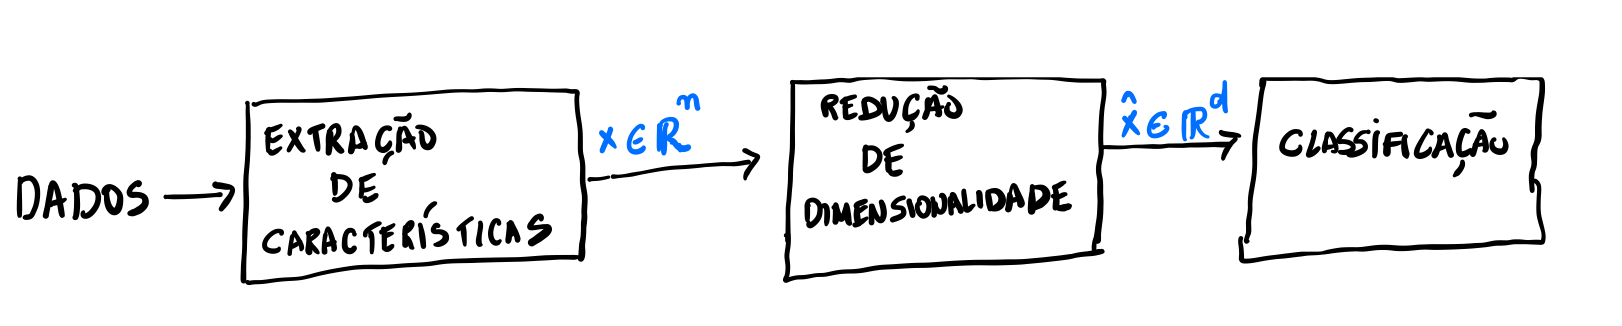
\includegraphics[scale=0.19]{./figs/PCA_Fig1.png}
\end{center}
}

\Sli{

\justifying Usualmente, em problemas de classificação, temos a impressão de, quanto mais características temos, melhor será a taxa de acerto de nossa técnica. No entanto, em problemas reais em que temos um número \textbf{limitado de amostras}, observa-se um fenômeno conhecido por \textbf{maldição da dimensionalidade.} Existe, então, uma série de efeitos negativos ocasionados pelo aumento indiscriminado de características:

\begin{itemize}
	\item \underline{Fenômeno de Hughes:} para um número finito de amostras, existe uma dimensionalidade $d^\ast$ que, após este valor, o desempenho da taxa de classificação diminui.
\end{itemize}

\begin{center}
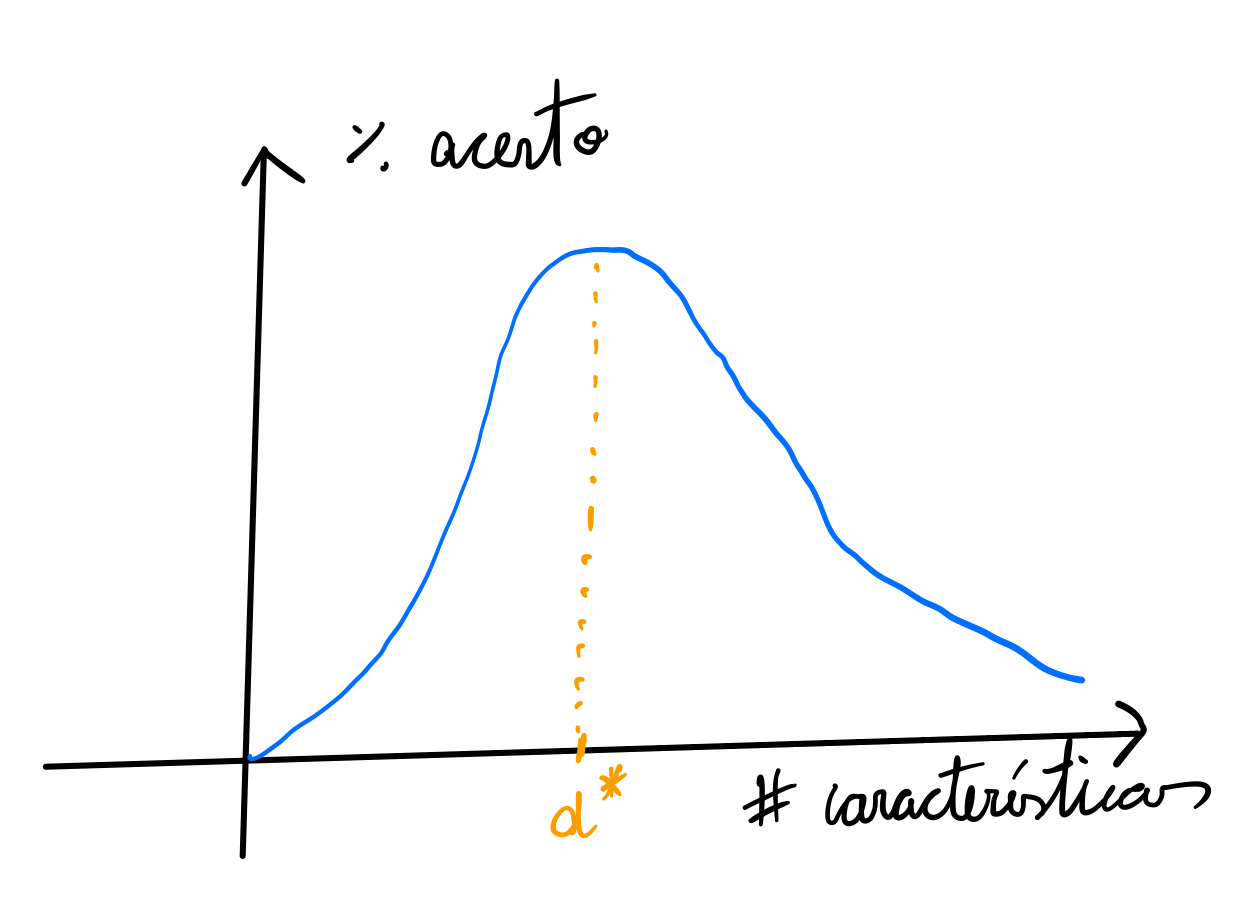
\includegraphics[scale=0.11]{./figs/PCA_Fig2.png}
\end{center}

%Análise de Componentes Principais, do inglês \emph{Principal Component Analysis} - PCA, 
}

\Sli{

\begin{itemize}
	\item \underline{Número de amostras como função das características:} em classificadores não paramétricos, o número de amostras deve ser uma função exponencial do número de características.
	\item \underline{Gaussianas multivariadas:} em distribuições Gaussianas multivariadas com alta dimensão, a densidade das amostras tende a se concentrar na cauda da distribuição, ou seja, longe da média amostral, dificultando a classificação.
\end{itemize}

\begin{center}
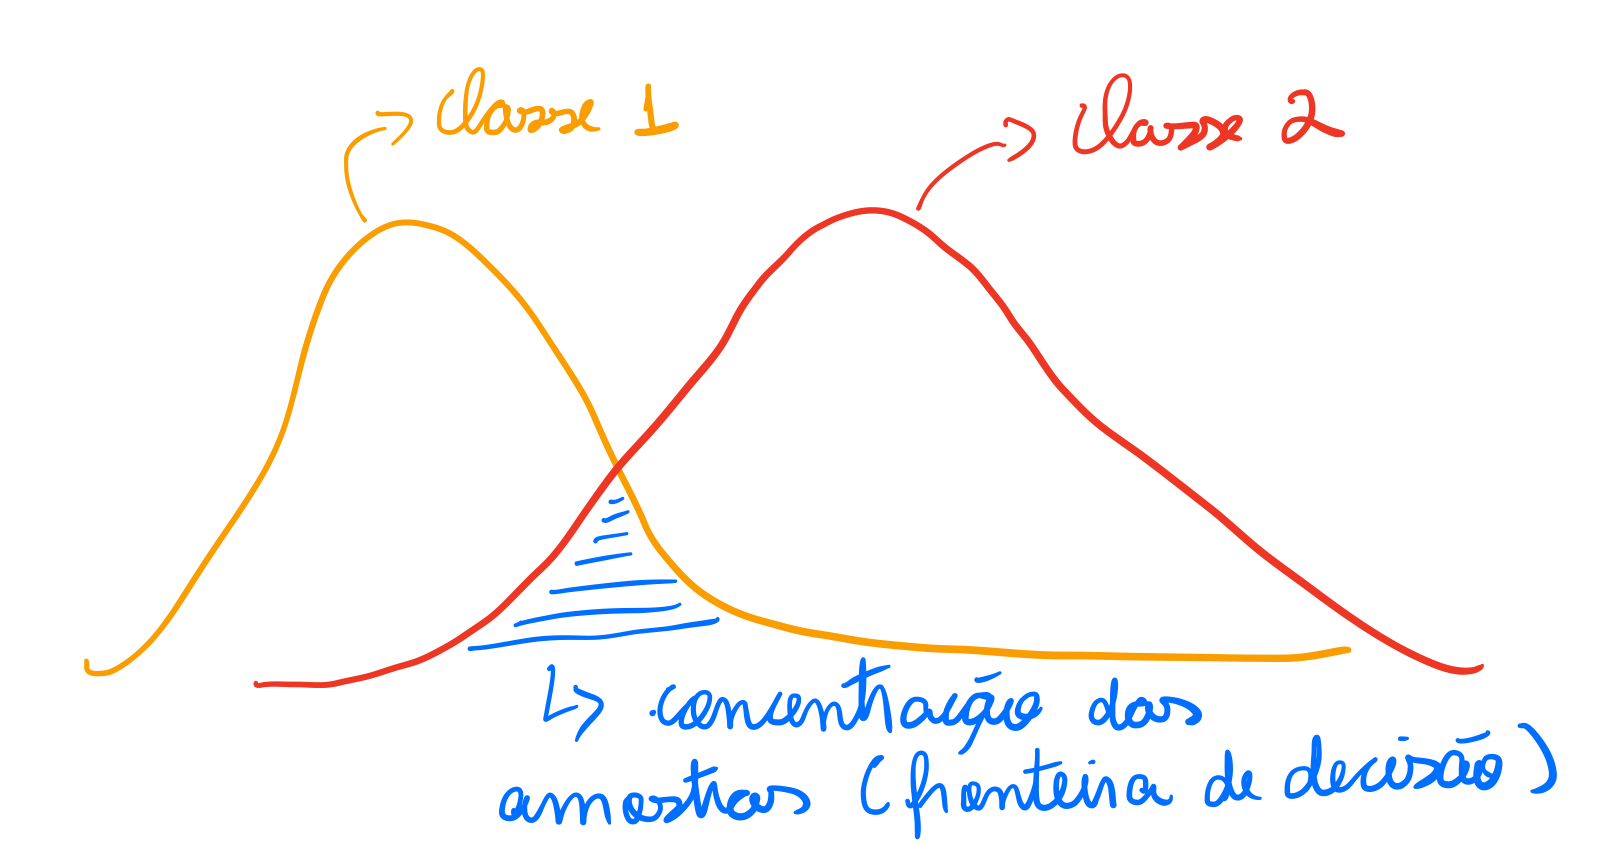
\includegraphics[scale=0.13]{./figs/PCA_Fig3.png}
\end{center}
}

\SliT{Autovalores e Autovetores: Uma Breve Introdução}{

\justifying Seja $V$ um espaço vetorial com $n$ dimensões que contempla um produto interno. Então, temos que:

\begin{equation}
	\langle \bm{u},\bm{v}\rangle = \bm{u}^T\bm{v} = \sum_{i=1}^nu_iv_i,
\end{equation}
e
\begin{equation}
	\langle \bm{v},\bm{v}\rangle = \bm{v}^T\bm{v} = \sum_{i=1}^nv_i = \norm{v}^2.
\end{equation}
}

\Sli{
\justifying Geometricamente falando, como vimos anteriormente, o produto interno entre os vetores $\bm{u}$ e $\bm{v}$ é a \textbf{projeção} de $\bm{u}$ em $\bm{v}$.

\begin{center}
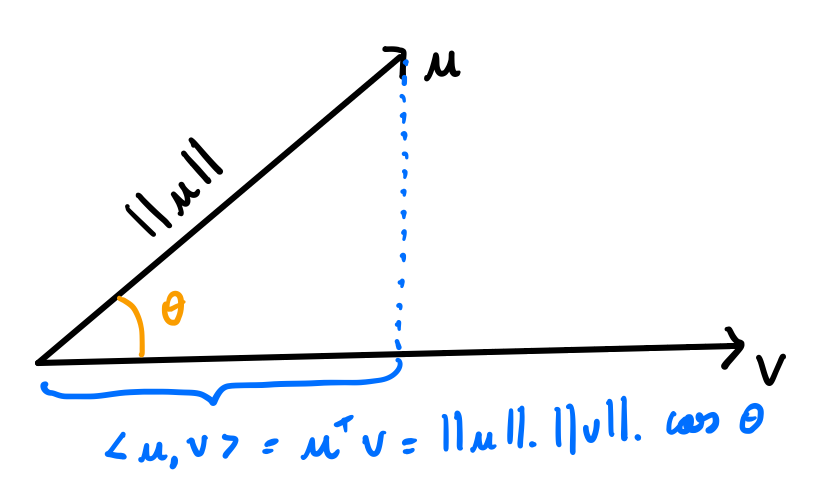
\includegraphics[scale=0.19]{./figs/PCA_Fig4.png}
\end{center}

A ideia é que neste espaço vetorial eu consiga definir \textbf{operadores lineares}, ou seja, funções (matrizes) $\bm{P}$ que mapeiam vetores de entrada $\bm{v}$ em vetores de saída $\mu{u}$, ou seja:

\begin{equation}
	\bm{u} = \bm{P}\bm{v}.
\end{equation}
}

\Sli{
\justifying No estudo de autovalores e autovetores, estamos interessados em operadores lineares que possuem a seguinte característica: dado um operador linear $\bm{P}$ para quais vetores $\bm{v}$ a saída da Equação 3, ou seja, $\bm{u}$, aponta para a mesma direção da entrada, sendo apenas esticados ou encolhidos? Matematicamente falando, temos que:

\begin{equation}
	\bm{u} = \bm{P}\bm{v} = \lambda\bm{v}.
\end{equation}
\justifying Todos os vetores $\bm{v}$ que satisfazem a equação acima são chamados de \textbf{autovetores} de $\bm{P}$, e todos os escalares $\lambda$ que satisfazem a formulação acima são chamados de \textbf{autovalores} de $\bm{P}$. Na prática, $\lambda$ é um fator de escala de redução ou incremento do vetor $\bm{v}$. \underline{Assim sendo, dizemos} \underline{que $\bm{v}\in\mathbb{R}^n$ é um autovetor de $\bm{P}\in\mathbb{R}^{n\times n}$ com autovalor $\lambda$ se $\bm{v}\neq0$ e $\bm{P}\bm{v} = \lambda\bm{v}$}.
}

\Sli{
\justifying Para fins de explicação, tomemos o seguinte exemplo: seja $\bm{P} = \bm{I}\in\mathbb{R}^{n\times n}$ o operador identidade. Então, $\bm{I}\bm{v} = 1\bm{v}$, $\forall \bm{v}\in\mathbb{R}^n$. Desta forma, $\bm{v}$ é um autovetor de $\bm{I}$ com autovalor $\lambda=1$. Vejamos um outro exemplo, o operador de projeção em $\mathbb{R}^2$.

\begin{minipage}{0.42\textwidth}
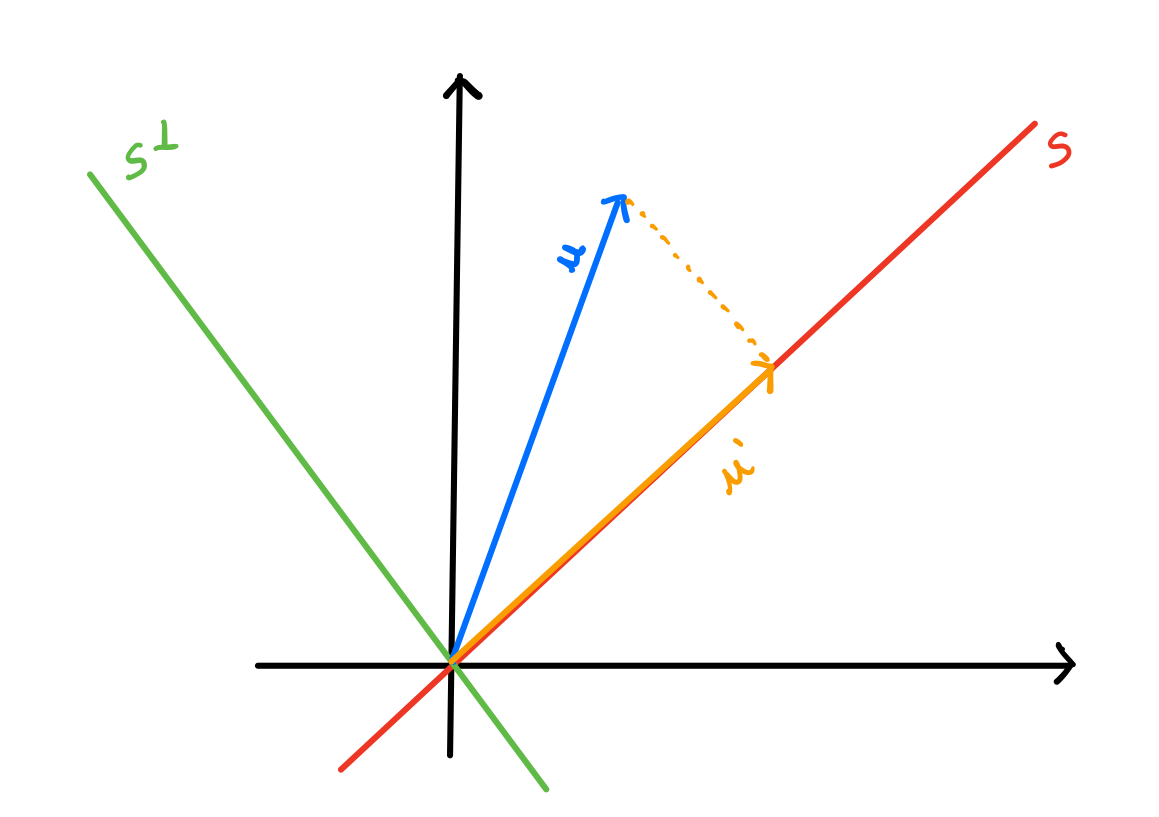
\includegraphics[scale=0.15]{./figs/PCA_Fig5.png}
\end{minipage}%%% to prevent a space
\begin{minipage}{0.57\textwidth}
\justifying Podemos definir o operador $\bm{P}_S$, o qual projeta o vetor $\bm{u}$ no subespaço (reta) $S$:

\begin{equation}
	\bm{u}^\prime= \bm{P}_S\bm{u}.
\end{equation}
Supondo um vetor $\bm{w}\in{S}$, temos que $\bm{w} = \bm{P}_S\bm{w}$, dado que $\bm{w}$ já faz parte do subespaço $S$. Neste caso, todo vetor que pertence à reta $S$ é um autovetor de $\bm{P}_S$ com autovalor $\lambda=1$.
\null
\par\xdef\tpd{\the\prevdepth}
\end{minipage}
 Seja, agora, $S^\perp$ o subespaço ortogonal a $\bm{S}$, e $\bm{x}\in S^\perp$, ou seja, quando eu aplicar o operador $\bm{P}_S$ em algum elemento de $\bm{S}$, resulta no valor $0$ (origem). Então, temos que $\bm{P}_S\bm{x} = 0\bm{x}$, ou seja, todo vetor que pertence a $S^\perp$ é um autovetor de $\bm{P}_S$ com autovalor $\lambda=0$.
}

\Sli{
\justifying Podemos extrapolar esse arcabouço de autovetores e autovalores para matrizes. Por exemplo, como podemos calcular os autovalores e autovetores de uma matrix $\bm{A}$? Da Equação 4, temos que:

\begin{equation}\nonumber
	\bm{A}\bm{v} = \lambda\bm{v}.
\end{equation}	
Rearranjando os temos, temos:
\begin{equation}
	\bm{A}\bm{v} - \lambda\bm{I}\bm{v} = 0\implies (\bm{A}- \lambda\bm{I})\bm{v} = 0.
\end{equation}
Existe um teorema da álgebra linear que nos diz o seguinte: $\bm{A}\bm{v} = 0$ admite solução não nula se, e somente se, $det(\bm{A}) = 0$. Assim, $det(\bm{A}- \lambda\bm{I}) = 0$ em nosso caso.
}

\Sli{
Ex: seja a matriz:
\begin{equation}\nonumber
\bm{A}=	\begin{bmatrix}
		3/2&-1/2\\
		-1/2&3/2
		\end{bmatrix}.
\end{equation}

Temos que: 
\begin{align}\nonumber
\bm{A}-\lambda\bm{I} &=	\begin{bmatrix}
		3/2&-1/2\\
		-1/2&3/2
		\end{bmatrix}-\lambda\begin{bmatrix}
		1&0\\
		0&1
		\end{bmatrix}\\\nonumber
		&= \begin{bmatrix}
		3/2-\lambda&-1/2\\
		-1/2&3/2-\lambda
		\end{bmatrix}.
\end{align}
}

\Sli{
Sabemos que $det(\bm{A}- \lambda\bm{I}) = 0$, ou seja:

\begin{equation}\nonumber
	\left(\frac{3}{2}-\lambda\right)^2-\left(-\frac{1}{2}*-\frac{1}{2}\right) = \left(\frac{3}{2}-\lambda\right)^2-\frac{1}{4} = 0,
\end{equation}
o que implica em:

\begin{equation}\nonumber
	\frac{9}{4}-2\frac{3}{2}\lambda+\lambda^2-\frac{1}{4} = 0\implies \lambda^2-3\lambda+2 = 0.
\end{equation}
Assim sendo, temos uma equação do segundo grau cujas soluções são $\lambda_1 = 1$ e $\lambda_2 = 2$.
}

\Sli{
Para obtermos o autovetor associado ao autovalor $\lambda_1 = 1$, temos que:

\begin{align}\nonumber
\bm{A}-\lambda\bm{I} &=	\begin{bmatrix}
		3/2&-1/2\\
		-1/2&3/2
		\end{bmatrix}-1\begin{bmatrix}
		1&0\\
		0&1
		\end{bmatrix}\\
		&= \begin{bmatrix}
		3/2-1&-1/2\\
		-1/2&3/2-1
		\end{bmatrix}\\\nonumber
		&= \begin{bmatrix}
		1/2&-1/2\\
		-1/2&1/2
		\end{bmatrix}.
\end{align}
}

\Sli{
Continuando, substituindo o resultado da Equação 7 na Equação 6, temos:

\begin{equation}\nonumber
	(\bm{A}-\lambda\bm{I})\bm{v} = 0
\end{equation}

\begin{equation}\nonumber
	\begin{bmatrix}
		1/2&-1/2\\
		-1/2&1/2
		\end{bmatrix}\bm{v} = 0
\end{equation}

\begin{equation}\nonumber
		\begin{bmatrix}
		1/2&-1/2\\
		-1/2&1/2
		\end{bmatrix}\begin{bmatrix}
		v_1\\
		v_2
		\end{bmatrix} = \begin{bmatrix}
		0\\
		0
		\end{bmatrix}\implies \left\{
			\begin{array}{ll}
			\frac{1}{2}v_1-\frac{1}{2}v_2 = 0 & \\
			-\frac{1}{2}v_1+\frac{1}{2}v_2 = 0 &
		\end{array}\right.\implies v_1=v_2\implies \bm{v}^{(1)} 
\end{equation}
Desta forma, $\bm{v}^{(1)}$ é o autovetor associado ao autovalor $\lambda_1$. 
}

\Sli{
\justifying Note que temos infinitos autovetores associadores ao autovalor $\lambda_1$, basta apenas que as componentes tenham o mesmo valor. Ex: $\bm{v}^{(1)}= \begin{bmatrix}
		1\\
		1
		\end{bmatrix}$ ou $\bm{v}^{(1)}= \begin{bmatrix}
		7\\
		7
		\end{bmatrix}$. Qual a diferença entre eles? \textbf{Todos apontam para a mesma direção, mas possuem magnitudes diferentes.} \newline

\justifying Usualmente, utilizamos o \textbf{autovetor canônico}, ou seja, aquele que tem \textbf{norma unitária}. Basta tomarmos um autovetor qualquer e dividirmos cada componente pela sua norma, ou seja:

\begin{equation}\nonumber
	\bm{v}^{(1)}= 
	\begin{bmatrix}
		1\\
		1
		\end{bmatrix}\implies\bm{v}^{(1)}= 
		\begin{bmatrix}
		\frac{1}{\norm{\bm{v}^{(1)}}}\\
		\frac{1}{\norm{\bm{v}^{(1)}}}
		\end{bmatrix}\implies\bm{v}^{(1)}= 
		\begin{bmatrix}
		\frac{1}{\sqrt{2}}\\
		\frac{1}{\sqrt{2}}
		\end{bmatrix}.
\end{equation}
}

\Sli{
Agora, repetimos o processo para o autovalor $\lambda_2 = 0$:

\begin{equation}\nonumber
		\begin{bmatrix}
		-1/2&-1/2\\
		-1/2&-1/2
		\end{bmatrix}\begin{bmatrix}
		v_1\\
		v_2
		\end{bmatrix} = \begin{bmatrix}
		0\\
		0
		\end{bmatrix}\implies \left\{
			\begin{array}{ll}
			-\frac{1}{2}v_1-\frac{1}{2}v_2 = 0 & \\
			-\frac{1}{2}v_1-\frac{1}{2}v_2 = 0 &
		\end{array}\right.\implies v_1=-v_2\implies \bm{v}^{(2)}. 
\end{equation}
Novamente, utilizamos o autovetor canônico:
\begin{equation}\nonumber
	\bm{v}^{(2)}= 
	\begin{bmatrix}
		1\\
		1
		\end{bmatrix}\implies\bm{v}^{(2)}= 
		\begin{bmatrix}
		\frac{1}{\norm{\bm{v}^{(1)}}}\\
		-\frac{1}{\norm{\bm{v}^{(1)}}}
		\end{bmatrix}\implies\bm{v}^{(2)}= 
		\begin{bmatrix}
		\frac{1}{\sqrt{2}}\\
		-\frac{1}{\sqrt{2}}
		\end{bmatrix}.
\end{equation}
}

\Sli{
Desta forma, temos que $\bm{v}^{(1)}$ e $\bm{v}^{(2)}$ são os nossos autovetores do operador linear $\bm{P}_S$. Geometricamente falando, temos o seguinte:

\begin{minipage}{0.42\textwidth}
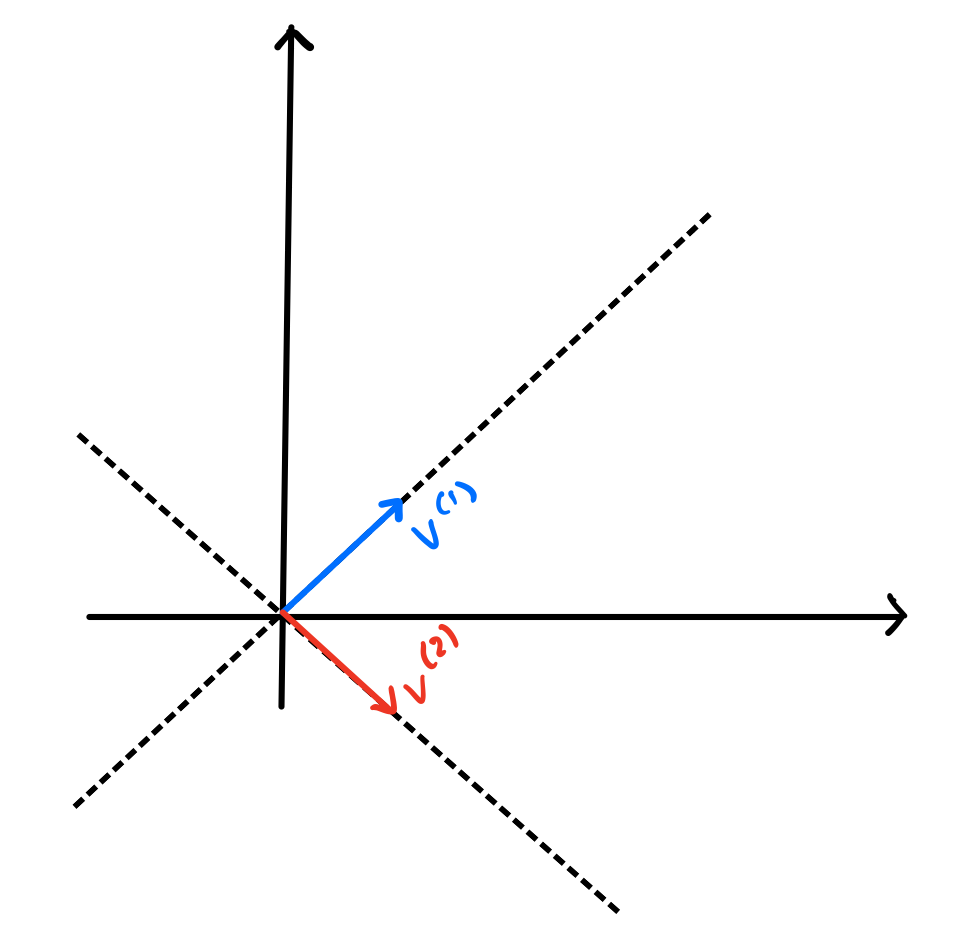
\includegraphics[scale=0.15]{./figs/PCA_Fig6.png}
\end{minipage}%%% to prevent a space
\begin{minipage}{0.57\textwidth}
\justifying Temos que os autovetores definem uma nova base no sistema de coordenadas. Existe um teorema que nos diz o seguinte: ``Se $\bm{P}$ é um operador linear que possui $n$ autovalores distintos, então os autovetores de $\bm{P}$ definem uma nova base em $\mathbb{R}^n$."
\null
\par\xdef\tpd{\the\prevdepth}
\end{minipage}
}

\Sli{
\justifying Podemos organizar os autovetores em uma matriz $\bm{Q}$ da seguinte forma:

\begin{equation}\nonumber
	\bm{Q} = \begin{bmatrix}
		\bm{v}^{(1)} & \bm{v}^{(2)} & \ldots & \bm{v}^{(n)}.
	\end{bmatrix}
\end{equation}
Ademais, temos que uma matriz é dita ser \textbf{positiva semidefinida} se todos os seus autovalores foram maiores ou iguais a $0$. Temos, ainda, uma outra definição: ``Seja $\bm{P}$ um operador linear. Caso a matriz $\bm{Q}$ dos seus autovetores defina uma nova base em $\mathbb{R}^n$, então $\bm{P}\bm{Q}=\bm{Q}\bm{\Lambda}$, em que $\bm{\Lambda}$ representa a matriz diagonal dos autovalores".

\justifying Um outro teorema fundamental (decomposição expectral) nos diz que: ``Seja $\bm{P}$ uma matriz quadrada $n\times n$, $\bm{Q}$ a sua matriz de autovetores (nas colunas) e $\bm{\Lambda}$ a sua matriz diagonal de autovalores. Então, temos que  a matriz $\bm{P}$ pode ser decomposta da seguinte forma:"

\begin{equation}
	\bm{P} = \bm{Q}\bm{\Lambda}\bm{Q}^{-1}.
\end{equation}
Caso $\bm{P}$ seja ortogonal (ex: matrizes de rotação do espaço), então $\bm{Q}^{-1} = \bm{Q}^T$. Desta forma, temos que $\bm{P} = \bm{Q}\bm{\Lambda}\bm{Q}^T$.
}

\SliT{Análise de Componentes Principais pela Maximização da Variância}{

\justifying A técnica PCA nos permite tratar dados de alta dimensionalidade identificando a dependência entre as variáveis para representá-los de uma forma mais compacta e minimizando a perda de informação relevante. É uma das técnicas mais utilizadas no contexto de \textbf{redução de características}. Possui outros nomes, tais como: (i) Transformação de Karhunen-Loeve, (ii) Transformação de Hotelling e (iii) Decomposição em Valores Singulares.
}

\Sli{
Características principais:

\begin{itemize}
	\item Transformação linear: assume a hipótese que os dados encontram-se em um subespaço Euclidiano de $\mathbb{R}^n$.
	\item Método não supervisionado.
	\item Decorrelaciona os dados de entrada eliminando redundâncias (a matriz de covariância dos dados transformados é diagonal).
\end{itemize}

\begin{equation}\nonumber
	\bm{x}\in\mathbb{R}^n\overset{\text{PCA}}{\implies}\hat{\bm{x}}\in\mathbb{R}^d
\end{equation}
Basicamente, queremos achar um operador que projete os dados de entrada em um espaço de saída com menor dimensão.
}

\Sli{
\justifying Seja $Z=[T^T,S^T]$ uma base ortonormal em $\mathbb{R}^n$, em que:

\begin{itemize}
	\item $T^T = [\bm{w}_1,\bm{w}_2,\ldots,\bm{w}_d]$ corresponde ao vetor de componentes que iremos \textbf{reter} no processo de redução e
	\item $S^T = [\bm{w}_{k+1},\bm{w}_{k+2},\ldots,\bm{w}_n]$ corresponde ao vetor de componentes que iremos \textbf{descartar}.
\end{itemize}
\justifying Desta forma, $T$ representa o novo sistema de eixos coordenados encontrados pelo PCA, enquanto que $S$ representa o subespaço eliminado durante o processo de redução.\newline

\justifying \underline{Problema:} dado um espaço de entrada, queremos encontrar as $d$ direções $\bm{w}_i$ que, ao projetarmos os dados, maximizam a variância (espalhamento) retida na nova representação.
}

\Sli{
\justifying Temos que nosso vetor $\bm{x}\in\mathbb{R}^n$ pode ser expandido em nossa base ortonormal da seguinte forma:

\begin{equation}
	\bm{x} = \sum_{j=1}^n(\bm{x}^T\bm{w}_j)\bm{w}_j = \sum_{j=1}^nc_j\bm{w}_j,
\end{equation}
em que $\bm{c}\in\mathbb{R}^n$ corresponde ao vetor de coeficientes de expansão.

\begin{minipage}{0.42\textwidth}
	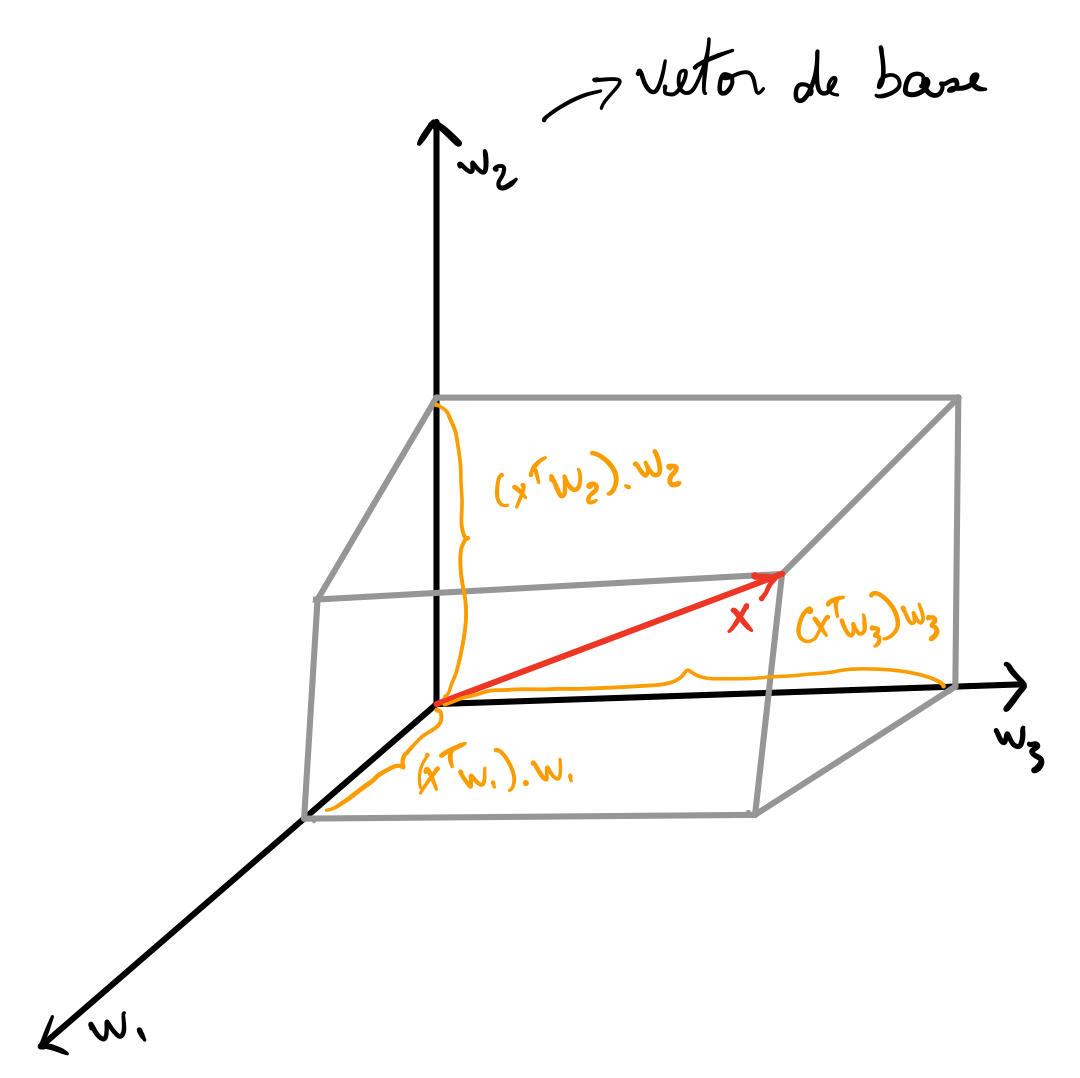
\includegraphics[scale=0.12]{./figs/PCA_Fig7.png}
\end{minipage}%%% to prevent a space
\begin{minipage}{0.57\textwidth}
\justifying Note que o termo $\bm{x}^T\bm{w}_j$ corresponde à projeção de $\bm{x}$ no vetor de base $\bm{w}_j$.
\null
\par\xdef\tpd{\the\prevdepth}
\end{minipage}
}

\Sli{
Temos que o vetor reduzido para o novo espaço pode ser calculado da seguinte forma:

\begin{equation}
	\hat{\bm{x}} = T\bm{x}\implies\hat{\bm{x}}^T = \bm{x}^TT^T = \sum_{j=1}^nc_j\bm{w}_j^TT^T.
\end{equation}
Note que a propriedade de ortonormalidade (bases ortonormais) nos diz que:

\begin{equation}
	\bm{w}_i^T\bm{w}_j = \begin{cases}
		1 & \text{se $i=j$}\\
		0 & \text{caso contrário.}
	\end{cases}
\end{equation}
Assim, podemos reescrever a Equação 10 conforme segue:

\begin{equation}
	\hat{\bm{x}} = \sum_{j=1}^nc_j\bm{w}_j^TT^T = \sum_{j=1}^nc_j\bm{w}_j^T[\bm{w}_1,\bm{w}_2,\ldots,\bm{w}_n] = [c_1,c_2,\ldots,c_n].
\end{equation}
}

\Sli{
\justifying Assim, queremos encontrar uma transformação $T$ (conjunto de componentes) que \textbf{maximize} a variância retida nos dados, ou seja, queremos maximizar a seguinte função:

\begin{equation}
	L(T) = E\left[\norm{\hat{\bm{x}}^2}\right] = \left[\hat{\bm{x}}^T\hat{\bm{x}}\right]=\sum_{j=1}^dE[c_j^2],
\end{equation}
lembrando que $\norm{\hat{\bm{x}}^2}$ corresponde à norma ao quadrado de $\bm{\hat{x}}$, ou seja, queremos obter novas componentes cujas normas (distâncias a partir da origem) sejam maximizadas, ou seja, estejam mais ``espalhadas". Note que $\left[\hat{\bm{x}}^T\hat{\bm{x}}\right] = E\left[\hat{x}_1^2\right] + E\left[\hat{x}_2^2\right]+\ldots+E\left[\hat{x}_d^2\right]$, ou seja, a soma das variâncias em cada eixo coordenado da nova representação.
}

\Sli{
\justifying Da Equação 9, temos que $c_j = \bm{x}^T\bm{w}_j$. Assim, substuindo-se $c_j$ na Equação 13, temos que:

\begin{align}\nonumber
	L(T) &= \sum_{i=1}^dE[c_j^2] = \sum_{i=1}^dE[(\bm{x}^T\bm{w}_j)^2]\\
		&= \sum_{i=1}^dE[\bm{w}_i^T\bm{x}\bm{x}^T\bm{w}_i] = \sum_{i=1}^d\bm{w}_i^TE[\bm{x}\bm{x}^T]\bm{w}_i\\\nonumber
		&= \sum_{i=1}^d\bm{w}_i^T\Sigma_{\bm{x}}\bm{w}_i,
\end{align}
em que $\Sigma_{\bm{x}}$ corresponde à matrix de covariância dos dados observados, ou seja, do vetor de entrada $\bm{x}$. Ademais, temos que a Equação 14 está sujeita à restrição $\norm{\bm{w}_i}^2 = 1$.
}

\Sli{
\justifying Desta forma, o problema de otimização consiste em: 

\begin{equation}
	\bm{w}^\ast = \argmax_{\bm{w}}\sum_{i=1}^d\bm{w}_i^T\Sigma_{\bm{x}}\bm{w}_i,
\end{equation}
sujeito à $\norm{\bm{w}_i}^2 = 1$, $\forall i = 1,2\ldots,d$. Desta forma, nosso problema consiste em encontrar as $d$ direções ortogonais $\bm{w}_i$ que maximizam o somatório acima. Note que o somatório contém a matriz de covariância dos dados, ou seja, queremos maximizar a sua variância nessas direções ortogonais.\newline

\justifying Temos, então, um problema de otimização com restrições de desigualdade, ou seja, precisamos fazer uso da técnica de Multiplicadores de Lagrange.
}

\Sli{
\justifying Escrevendo a Equação 14 de acordo com os Multiplicadores de Lagrange, temos que:

\begin{equation}
	L(T,\bm{\alpha}) = \sum_{i=1}^d\bm{w}_i^T\Sigma_{\bm{x}}\bm{w}_i-\sum_{i=1}^d\alpha_i(\underbrace{\bm{w}_i^T\bm{w}_i-1}_{\norm{\bm{w}}^2=1}).
\end{equation}
Como queremos maximizar a equação acima visando cada $\bm{w}_i$, basta, então, calcularmos a derivada de $L(T,\bm{\alpha})$ em relação à $\bm{w}_i$ e igualarmos à 0, ou seja:

\begin{equation}
\frac{\partial L(T,\bm{\alpha})}{\partial \bm{w}_i} = \bm{\Sigma_{\bm{x}}}\bm{w}_i-\alpha_i\bm{w}_i = 0	\implies\bm{\Sigma_{\bm{x}}}\bm{w}_i = \alpha_i\bm{w}_i.
\end{equation}
\justifying O resultado da equação acima nos leva à formulação do problema de encontrar os autovalores e autovetores. \textbf{Assim, as direções $\bm{w}_i$ são os autovetores da matriz de covariância dos dados de entrada.}
}

\Sli{
\justifying Podemos reescrever a Equação 15 da seguinte forma:

\begin{align}\nonumber
	\bm{w}^\ast &= \argmax_{\bm{w}}\sum_{i=1}^d\bm{w}_i^T\Sigma_{\bm{x}}\bm{w}_i = \argmax_{\bm{w}}\sum_{i=1}^d\bm{w}_i^T\alpha_i\bm{w}_i\\
	&= \argmax_{\bm{w}}\sum_{i=1}^d\alpha_i\cancelto{1}{\norm{\bm{w}_i}^2} = \argmax_{\bm{w}}\sum_{i=1}^d\alpha_i.\\\nonumber
\end{align}
A equação acima nos diz que devemos maximizar o somatório dos $d$ autovalores. \underline{Isto define o} \underline{nosso problema, ou seja, encontrar as $d$ direções que maximizam a variância dos dados!}
}

\end{document}